\chapter{XBee}
\label{cha:XBee}

\section{ZigBee模块概述}

无线通信协议是在无线设备之间进行数据交换的一组规则。RF模块根据模块及其无线固件支持特定的无线通信协议。

以下是XBee无线模块支持的协议的完整列表:

\begin{itemize}
    \item IEEE 802.15.4
    \item ZigBee
    \item ZigBee Smart Energy
    \item DigiMesh (Digi proprietary)
    \item ZNet
    \item IEEE 802.11 (Wi-Fi)
    \item Point-to-multipoint (Digi proprietary)
    \item XSC (XStream-compatible)
\end{itemize}

\begin{figure}[htbp]
    \centering
    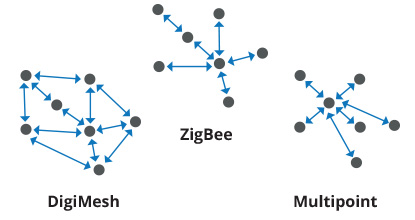
\includegraphics[width=0.5\columnwidth]{radio_comm_protocols.png}
    \caption{不同协议组网方式对比}
    \label{fig:radio_comm_protocols}
\end{figure}

并非所有XBee设备都可以运行所有列出的通信协议。XBee硬件和无线固件的组合决定了XBee设备可以执行的协议。

\begin{figure}[htbp]
    \centering
    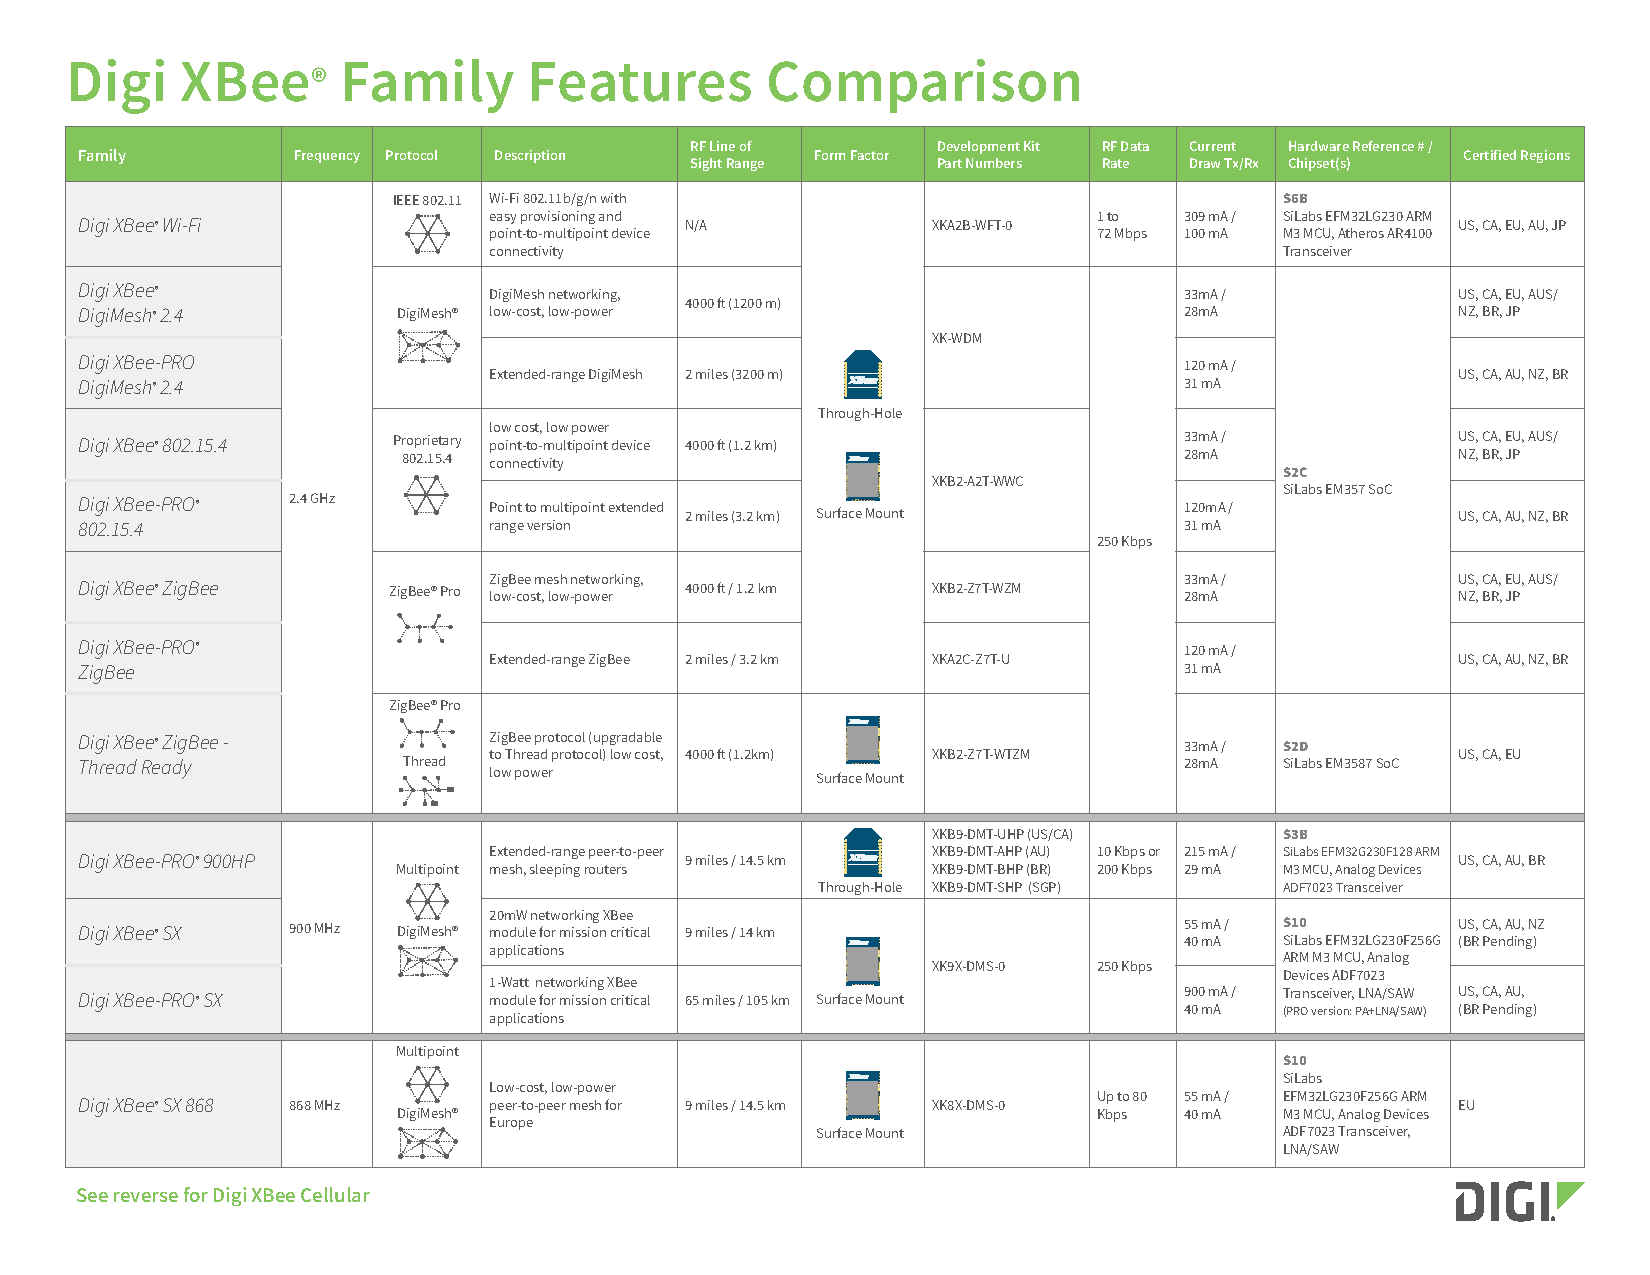
\includegraphics[width=\columnwidth]{chart_xbee_rf_features.pdf}
    \caption{Digi XBee Family Features Comparison}
    \label{fig:xbee_rf_features}
\end{figure}

\section{固件升级}

本地设备设置AP=2 即 API mode 能使用Network Working Mode,以便升级固件。

用XBee 3 无线连接淘宝买的XBee Pro S2B需要先下载lagacy XBee Firmware。但不能直接无线更新固件,还是需要用USB连接到电脑上烧写新固件。XBee3则可以直接无线更新。

这就决定了小车上尽可能使用XBee3,虽然要比XBee S2B贵3-4倍。当然也可以直接在我们的PCB上画FT232接USB口以便更新固件使用,或者预留编程口直接使用编程线。

只有以下这些模块才能无线更新固件:

\begin{itemize}
    \item XBee/XBee PRO SX
    \item XLR Pro Module
    \item XBee/XBee PRO 802.15.4 (S2C module versions only)
    \item XBee/XBee-PRO DigiMesh 2.4 (S2C module versions only)
    \item XTend RF Module Family (SX module versions only)
    \item XBee/XBee-PRO ZB and Programmable XBee-PRO ZB
    \item XBee/XBee-PRO ZB SMT and Programmable XBee-PRO ZB SMT
    \item XBee-PRO 900HP and Programmable XBee-PRO 900HP
    \item XBee 865LP and Programmable XBee 865LP
    \item XBee3 (Zigbee, DigiMesh 2.4, and 802.15.4)
\end{itemize}

\section{AP参数}

XBee无线模块的操作模式建立了用户或连接到XBee的任何微控制器通过UART或串行接口与模块进行通信的方式。

取决于固件及其配置,无线模块可以在三种不同的操作模式下工作:

\begin{itemize}
    \item Application Transparent (AT) operating mode
    \item API operating mode
    \item API escaped operating mode
\end{itemize}

在某些情况下,无线模块的运行模式由固件版本(确定运行模式是AT还是API)以及固件的AP设置(确定API模式)决定。在其他情况下,操作模式仅由AP设置确定,该设置允许将模式配置为AT(AP = 0),API(AP = 1)或API Escape(AP = 2)。

\section{AT Mode}

在AT (Application Transparent) 透明操作模式下,无线模块接收的所有串行数据都排队等待RF传输。当模块接收到RF数据时,数据将通过串行接口发送出去。

要配置在AT中运行的XBee模块,必须将其置于命令模式下以发送配置命令。

当无线模块在AT工作模式下工作时,必须使用命令模式 command mode 界面来配置设置。

要进入AT命令模式,在一秒钟内发送三个字符的命令序列(通常为"+++")。一旦启动了AT命令模式,该模块将发送"OK \\ r",启动命令模式计时器,并且无线模块能够接收AT命令。

AT命令的结构为:

\begin{tcolorbox}
    AT[ASCII command][Space (optional)][Parameter (optional)][Carriage return]
\end{tcolorbox}

例如:

\begin{tcolorbox}
    ATNI MyDevice\textbackslash{}r
\end{tcolorbox}

如果在命令模式超时内未收到有效的AT命令,则无线模块将自动退出AT命令模式。还可以通过发出CN命令来退出命令模式:

\begin{tcolorbox}
    (ATCN\textbackslash{}r)
\end{tcolorbox}

\section{XBee API Mode}

API(Application Programming Interface 应用程序编程接口)操作模式是AT模式的替代。API操作模式要求通过结构化接口与模块进行通信。换句话说,数据通过API框架进行通信。如图~\ref{fig:xbee_api_transmission}。

\subsection{API Mode 概述}

API指定了如何使用串行接口从模块发送和接收命令,命令响应和模块状态消息。使用API​​操作模式,可以:

\begin{itemize}
    \item 配置本地XBee模块。
    \item 在网络中配置远程模块。
    \item 管理数据到多个目的地的传输。
    \item 接收每个发送的射频数据包的成功/失败状态。
    \item 标识每个接收到的数据包的源地址。
    \item 获取任何接收到的数据包的信号强度。
    \item 执行高级网络管理和诊断。
    \item 执行高级功能,例如远程固件更新,ZDO,ZCL等。
\end{itemize}

\begin{figure}[htbp]
    \centering
    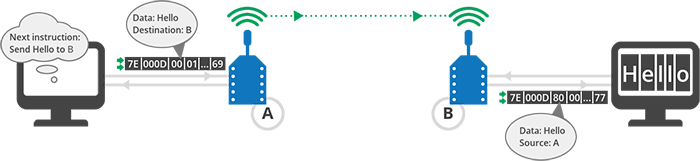
\includegraphics[width=\columnwidth]{xbee_api_transmission.png}
    \caption{API模式传输数据}
    \label{fig:xbee_api_transmission}
\end{figure}


取决于AP参数值,无线模块可以以下两种模式之一运行:API(AP = 1)或API Escape(AP = 2)操作模式。

API转义操作模式(AP = 2)与API模式相似,不同之处在于,在API转义模式下工作时,必须转义API框架特定数据的某些字节。由于XCTU与API和API转义操作模式均兼容,因此无需手动转义字符。

API转义操作模式通过防止与特殊字符(例如帧开始字节(0x7E))发生冲突,提高了RF传输的可靠性。API非转义(API = 1)操作仅依靠起始定界符和长度字节来区分API帧。另一方面,在API转义模式下,那些特殊字节被转义。由于0x7E只能出现在API数据包的开头,因此,如果在处于API转义模式下的任何时间接收到0x7E,则模块始终可以“假定”新数据包已经开始。

在以API转义模式发送或接收API帧时,必须对特定数据值进行转义(标记),以免干扰数据帧序列。

要转义数据字节,请插入0x7D,然后在其后跟要转义的字节与0x20进行XOR。需要转义的数据字节如下:

\begin{itemize}
    \item 0x7E: Frame delimiter
    \item 0x7D: Escape
    \item 0x11: XON
    \item 0x13: XOFF    
\end{itemize}

XCTU在与API转义的无线电模块进行交互时会自动转义适当的字符。

\subsection{APT frame structure 数据包结构}

API帧是在无线电模块的串行接口上​​以API或API转义操作模式进行配置时发送和接收的结构化数据。API框架用于与模块或网络中的其他模块进行通信。

API模式下的结构化数据包称为帧。 它们通过设备的串行接口发送和接收,并且包含无线消息本身以及一些额外的信息,例如数据的目标/源或信号质量。

当设备处于API模式时,所有通过串行接口进入和离开模块的数据都包含在框架中,这些框架定义了设备内的操作或事件。

API帧具有图~\ref{fig:api-frame}和表~\ref{tab:API-frame-structure}所示的结构:

开始符 Start delimeter 帧的第一个字节,由一个特殊的比特序列组成,这些比特序列指示数据帧的开始。它的值始终为0x7E。作用是检测新的输入帧。

长度 Length 指定帧数据字段中包含的字节总数。它的两个字节的值不包括起始符,长度和校验和。

帧数据 Frame data 由API标识符和特定于API标识符的数据组成。特定数据的内容取决于API标识符(也称为API帧类型)。

校验和 Checksum 帧的最后一个字节。它有助于测试数据的完整性,并通过获取其之前所有API帧字节(不包括前三个字节(开始符和长度))的哈希总和来计算。

\begin{figure}[htbp]
    \centering
    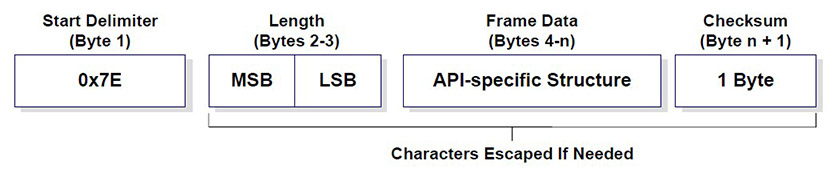
\includegraphics[width=\columnwidth]{concpts_api_frame_explained_80.jpg}
    \caption{API帧}
    \label{fig:api-frame}
\end{figure}

\begin{table}[htbp]
    \centering
    \begin{tabular}{l|l|l|l|l|l|l|l|l|l|l|l} 
    \toprule
    Startdelimiter & \multicolumn{2}{l|}{~Length} & \multicolumn{8}{l|}{Frame data}                              & ~Checksum   \\ 
    \cline{4-11}
                   & \multicolumn{2}{l|}{}        & Frametype    & \multicolumn{7}{l|}{Data}                     &             \\ 
    \midrule
    1              & 2   & 3                      & 4            & 5 & 6 & 7 & 8 & 9 & ... & n                   & n+1         \\ 
    \cline{1-3}\cline{5-12}
    0x7E           & MSB & LSB                    & APIframetype & \multicolumn{7}{l|}{Frame-type-specific data} & Singlebyte  \\
    \bottomrule
    \end{tabular}
    \caption{API frame structure}
    \label{tab:API-frame-structure}
\end{table}

MSB 最高有效位(Most Significant Bit),在大端序中,MSB即指最左端的位。LSB(the least significant byte)则相反。

\subsection{API支持的Frame}

传输数据帧通过串行输入发送,数据将无线传输到远程XBees,如表~\ref{tab:XBee-Transmit-data-frames}。

% Please add the following required packages to your document preamble:
% \usepackage{booktabs}
\begin{table}[htbp]
    \begin{tabular}{@{}lll@{}}
    \toprule
    API ID & Frame name                        & Description                                                                                                       \\ \midrule
    0x08   & AT Command                        & Queries or sets parameters on the local XBee                                                                      \\
    0x09   & AT Command Queue Parameter Value  & Queries or sets parameters on the local XBee without applying changes                                             \\
    0x10   & Transmit Request                  & Transmits wireless data to the specified destination                                                              \\
    0x11   & Explicit Addressing Command Frame & Allows Zigbee application layer fields (endpoint and cluster ID) to be specified for a wireless data transmission \\
    0x17   & Remote AT Command Request         & Queries or sets parameters on the specified remote XBee module                                                    \\
    0x21   & Create Source Route               & Creates a source route in the module                                                                              \\
    0x24   & Register Joining Device           & Registers a module with the Trust Center                                                                          \\ \bottomrule
    \end{tabular}
    \caption{Transmit data frames 类型}
    \label{tab:XBee-Transmit-data-frames}
\end{table}

接收数据帧通过串行输出接收,数据从远程XBees无线接收,如表~\ref{tab:XBee-Receive-data-frames}。

% Please add the following required packages to your document preamble:
% \usepackage{booktabs}
\begin{table}[htbp]
    \begin{tabular}{@{}lll@{}}
    \toprule
    API ID & Frame name                          & Description                                                                                          \\ \midrule
    0x88   & AT Command Response                 & Displays the response to previous AT command frame                                                   \\
    0x8A   & Modem Status                        & Displays event notifications such as reset, association, disassociation, and so on.                  \\
    0x8B   & Transmit Status                     & Indicates wireless data transmission success or failure                                              \\
    0x90   & Receive Packet                      & Sends wirelessly received data out the serial interface (AO = 0)                                     \\
    0x91   & Explicit Rx Indicator               & Sends wirelessly received data out the serial interface when explicit mode is enabled (AO 0)         \\
    0x92   & IO Data Sample Rx Indicator         & Sends wirelessly received IO data out the serial interface                                           \\
    0x94   & XBee Sensor Read Indicator          & Sends wirelessly received sensor sample (from a Digi 1-wire sensor adapter) out the serial interface \\
    0x95   & Node Identification Indicator       & Displays received node identification message when explicit mode is disabled (AO = 0)                \\
    0x97   & Remote AT Command Response          & Displays the response to previous remote AT command requests                                         \\
    0x98   & Extended Modem Status               & Displays what is happening during the association when Verbose Join is enabled (DC10)                \\
    0xA0   & Over-the-Air Firmware Update Status & Provides a status indication of a firmware update transmission attempt                               \\
    0xA1   & Router Record Indicator             & Displays the multiple route hopes after a Zigbee route record command                                \\
    0xA3   & Many-to-One Route Request Indicator & Indicates a many-to-one route request is received                                                    \\
    0xA5   & Join Notification Status            & Indicates a module attempts to join, rejoin, or leave the network                                    \\ \bottomrule
    \end{tabular}
    \caption{Receive data frames 类型}
    \label{tab:XBee-Receive-data-frames}
\end{table}

\subsection{Frame Example}

以下发送和接收的API帧的示例以十六进制hexadecimal HEX格式表示。

示例:0x10-Transmit Request 发送请求

以下字符是发送请求帧:

7E 00 13 10 01 00 13 A2 00 40 DA 9D 23 A6 B9 00 00 48 65 6C 6C 6F 0C

\begin{itemize}
    \item 帧ID为0x01,因此发送方将接收带有发送结果的“发送状态”帧。
    \item 目标XBee具有64位地址00 13 A2 00 40 DA 9D 23和16位地址A6 B9。
    \item 没有指定任何选项。
    \item 要传输的数据是“ Hello”(48 65 6C 6C 6F)。
\end{itemize}

分析如表~\ref{tab:XBee-Frame-examples}。

% Please add the following required packages to your document preamble:
% \usepackage{booktabs}
% \usepackage{multirow}
\begin{table}[htbp]
    \begin{tabular}{@{}|l|l|l|l|l|@{}}
    \toprule
    \multicolumn{2}{|l|}{Frame fields} & Offset & Example & Description \\ \midrule
    \multicolumn{2}{|l|}{Start delimeter} & 0 & 0x7E &  \\ \midrule
    \multicolumn{2}{|l|}{\multirow{2}{*}{Length}} & MSB 1 & 0x00 & \multirow{2}{*}{Number of bytes between the length and the checksum} \\ \cmidrule(lr){3-4}
    \multicolumn{2}{|l|}{} & LSB 2 & 0x13 &  \\ \midrule
    \multirow{19}{*}{Frame data} & Frame type & 3 & 0x10 & 0x10 - Indicates this is a Transmit Request frame \\ \cmidrule(l){2-5} 
     & Frame ID & 4 & 0x01 & \begin{tabular}[c]{@{}l@{}}Identifies the data frame for the host to correlate with a subsequent Transmit Status (0x8B) frame.\\ Setting Frame ID to '0' will disable response frame.\end{tabular} \\ \cmidrule(l){2-5} 
     & \multirow{8}{*}{64-bit Destination address} & MSB 5 & 0x00 & \multirow{8}{*}{\begin{tabular}[c]{@{}l@{}}Set to the 64-bit address of the destination XBee\\ The following addresses are also supported:\\ 0x0000000000000000 - Coordinator address\\ 0x000000000000FFFF - Broadcast address\\ 0xFFFFFFFFFFFFFFFF - Unknown address if the destination's 64-bit address is unknown\end{tabular}} \\ \cmidrule(lr){3-4}
     &  & 6 & 0x13 &  \\ \cmidrule(lr){3-4}
     &  & 7 & 0xA2 &  \\ \cmidrule(lr){3-4}
     &  & 8 & 0x00 &  \\ \cmidrule(lr){3-4}
     &  & 9 & 0x40 &  \\ \cmidrule(lr){3-4}
     &  & 10 & 0xDA &  \\ \cmidrule(lr){3-4}
     &  & 11 & 0x9D &  \\ \cmidrule(lr){3-4}
     &  & LSB 12 & 0x23 &  \\ \cmidrule(l){2-5} 
     & \multirow{2}{*}{16-bit Destination address} & MSB 13 & 0xA6 & \multirow{2}{*}{\begin{tabular}[c]{@{}l@{}}Set to the 16-bit address of the destination XBee, if known.\\ The following addresses are also supported:\\ 0x0000 - Coordinator address\\ 0xFFFE - Unknwon address if the destination's 16-bit address is unknown, or if sending a broadcast\end{tabular}} \\ \cmidrule(lr){3-4}
     &  & LSB 14 & 0xB9 &  \\ \cmidrule(l){2-5} 
     & Broadcast Radius & 15 & 0x00 & \begin{tabular}[c]{@{}l@{}}Sets the maximum number of hops a broadcast transmission can occur. \\ If set to '0', the broadcast radius will be set to the maximum hops value.\end{tabular} \\ \cmidrule(l){2-5} 
     & Options & 16 & 0x00 & \begin{tabular}[c]{@{}l@{}}Bitfield of supported transmission options Supported values include the following:\\ 0x01 - Disable retries\\ 0x20 - Enable APS encryption (if EE = 1)\\ 0x40 - Use the extended transmission timeout for this destination\\ All other bits must be set to 0. \\ Enabling APS encryption decreases the maximum number of RF payload bytes by 4 (below the value reported by NP). \\ Setting the extended timeout bit causes the stack to set the extended transmission timeout for the destination address.\end{tabular} \\ \cmidrule(l){2-5} 
     & \multirow{5}{*}{RF Data} & MSB 14 & 0x48 & \multirow{5}{*}{Up to 255 bytes of data that is sent to the destination XBee} \\ \cmidrule(lr){3-4}
     &  & 15 & 0x65 &  \\ \cmidrule(lr){3-4}
     &  & ... & 0x6C &  \\ \cmidrule(lr){3-4}
     &  & 17 & 0x6C &  \\ \cmidrule(lr){3-4}
     &  & LSB 18 & 0x6F &  \\ \midrule
    \multicolumn{2}{|l|}{Checksum} & 22 & 0x6E & Hash sum of frame data bytes \\ \bottomrule
    \end{tabular}
    \caption{Frame examples}
    \label{tab:XBee-Frame-examples}
\end{table}

\subsection{AT和API模式对比}

API模式提供了一个结构化的接口,在该接口中,数据通过串行接口以有组织的数据包和确定的顺序进行通信。 这使可以在设备之间建立复杂的通信,而不必定义自己的协议。

默认情况下,XBee设备配置为在透传模式下工作:通过串行输入接收的所有数据都排队等待进行无线电传输,并且以无线方式接收的数据将按接收时的原样发送到串行输出,而没有其他信息。

因此,在透传模式下工作的设备有一些限制:

\begin{enumerate}
    \item 要在透传模式下读取或写入设备的配置,必须首先将设备转换为命令模式。
    \item 如果设备需要将消息传输到其他设备,则必须更新其配置以建立新的目的地。设备必须进入命令模式才能设置目标。
    \item 在透传模式下运行的设备无法识别其接收到的无线消息的来源。如果需要区分来自不同设备的数据,则发送设备必须包括所有设备已知的额外信息,以便以后可以提取。为此,必须定义一个鲁棒的协议,其中包括认为传输中需要的所有信息。
\end{enumerate}
 
由于透传模式的限制,设备提供了一种称为应用程序编程接口(API)的替代模式。 API模式提供了一个结构化的接口,在该接口中,数据通过串行接口以有组织的数据包和确定的顺序进行通信。这使无需定义自己的协议即可在模块之间建立复杂的通信。


API模式提供了一种执行以上所列操作的简便方法:

\begin{enumerate}
    \item 由于有不同的框架用于不同的目的(例如配置和通信),因此可以在不进入命令模式的情况下配置设备。
    \item 由于数据目标是API框架结构的一部分,因此可以使用API模式将消息传输到多个设备。
    \item API框架包括消息的来源,因此很容易识别数据的来源。    
\end{enumerate}

\section{使用XCTU API Mode 收发数据}

本节介绍如何使用XCTU控制台将数据传输到另一个XBee模块。 这些步骤包括使用要发送到其他模块的消息创建一个“发送请求”帧,并将该帧串行发送到本地XBee模块。可以在本地和远程模块中分析响应。如图~\ref{fig:XBee-XTCU-Send-Frame}。

\begin{figure}[htbp]
    \centering
    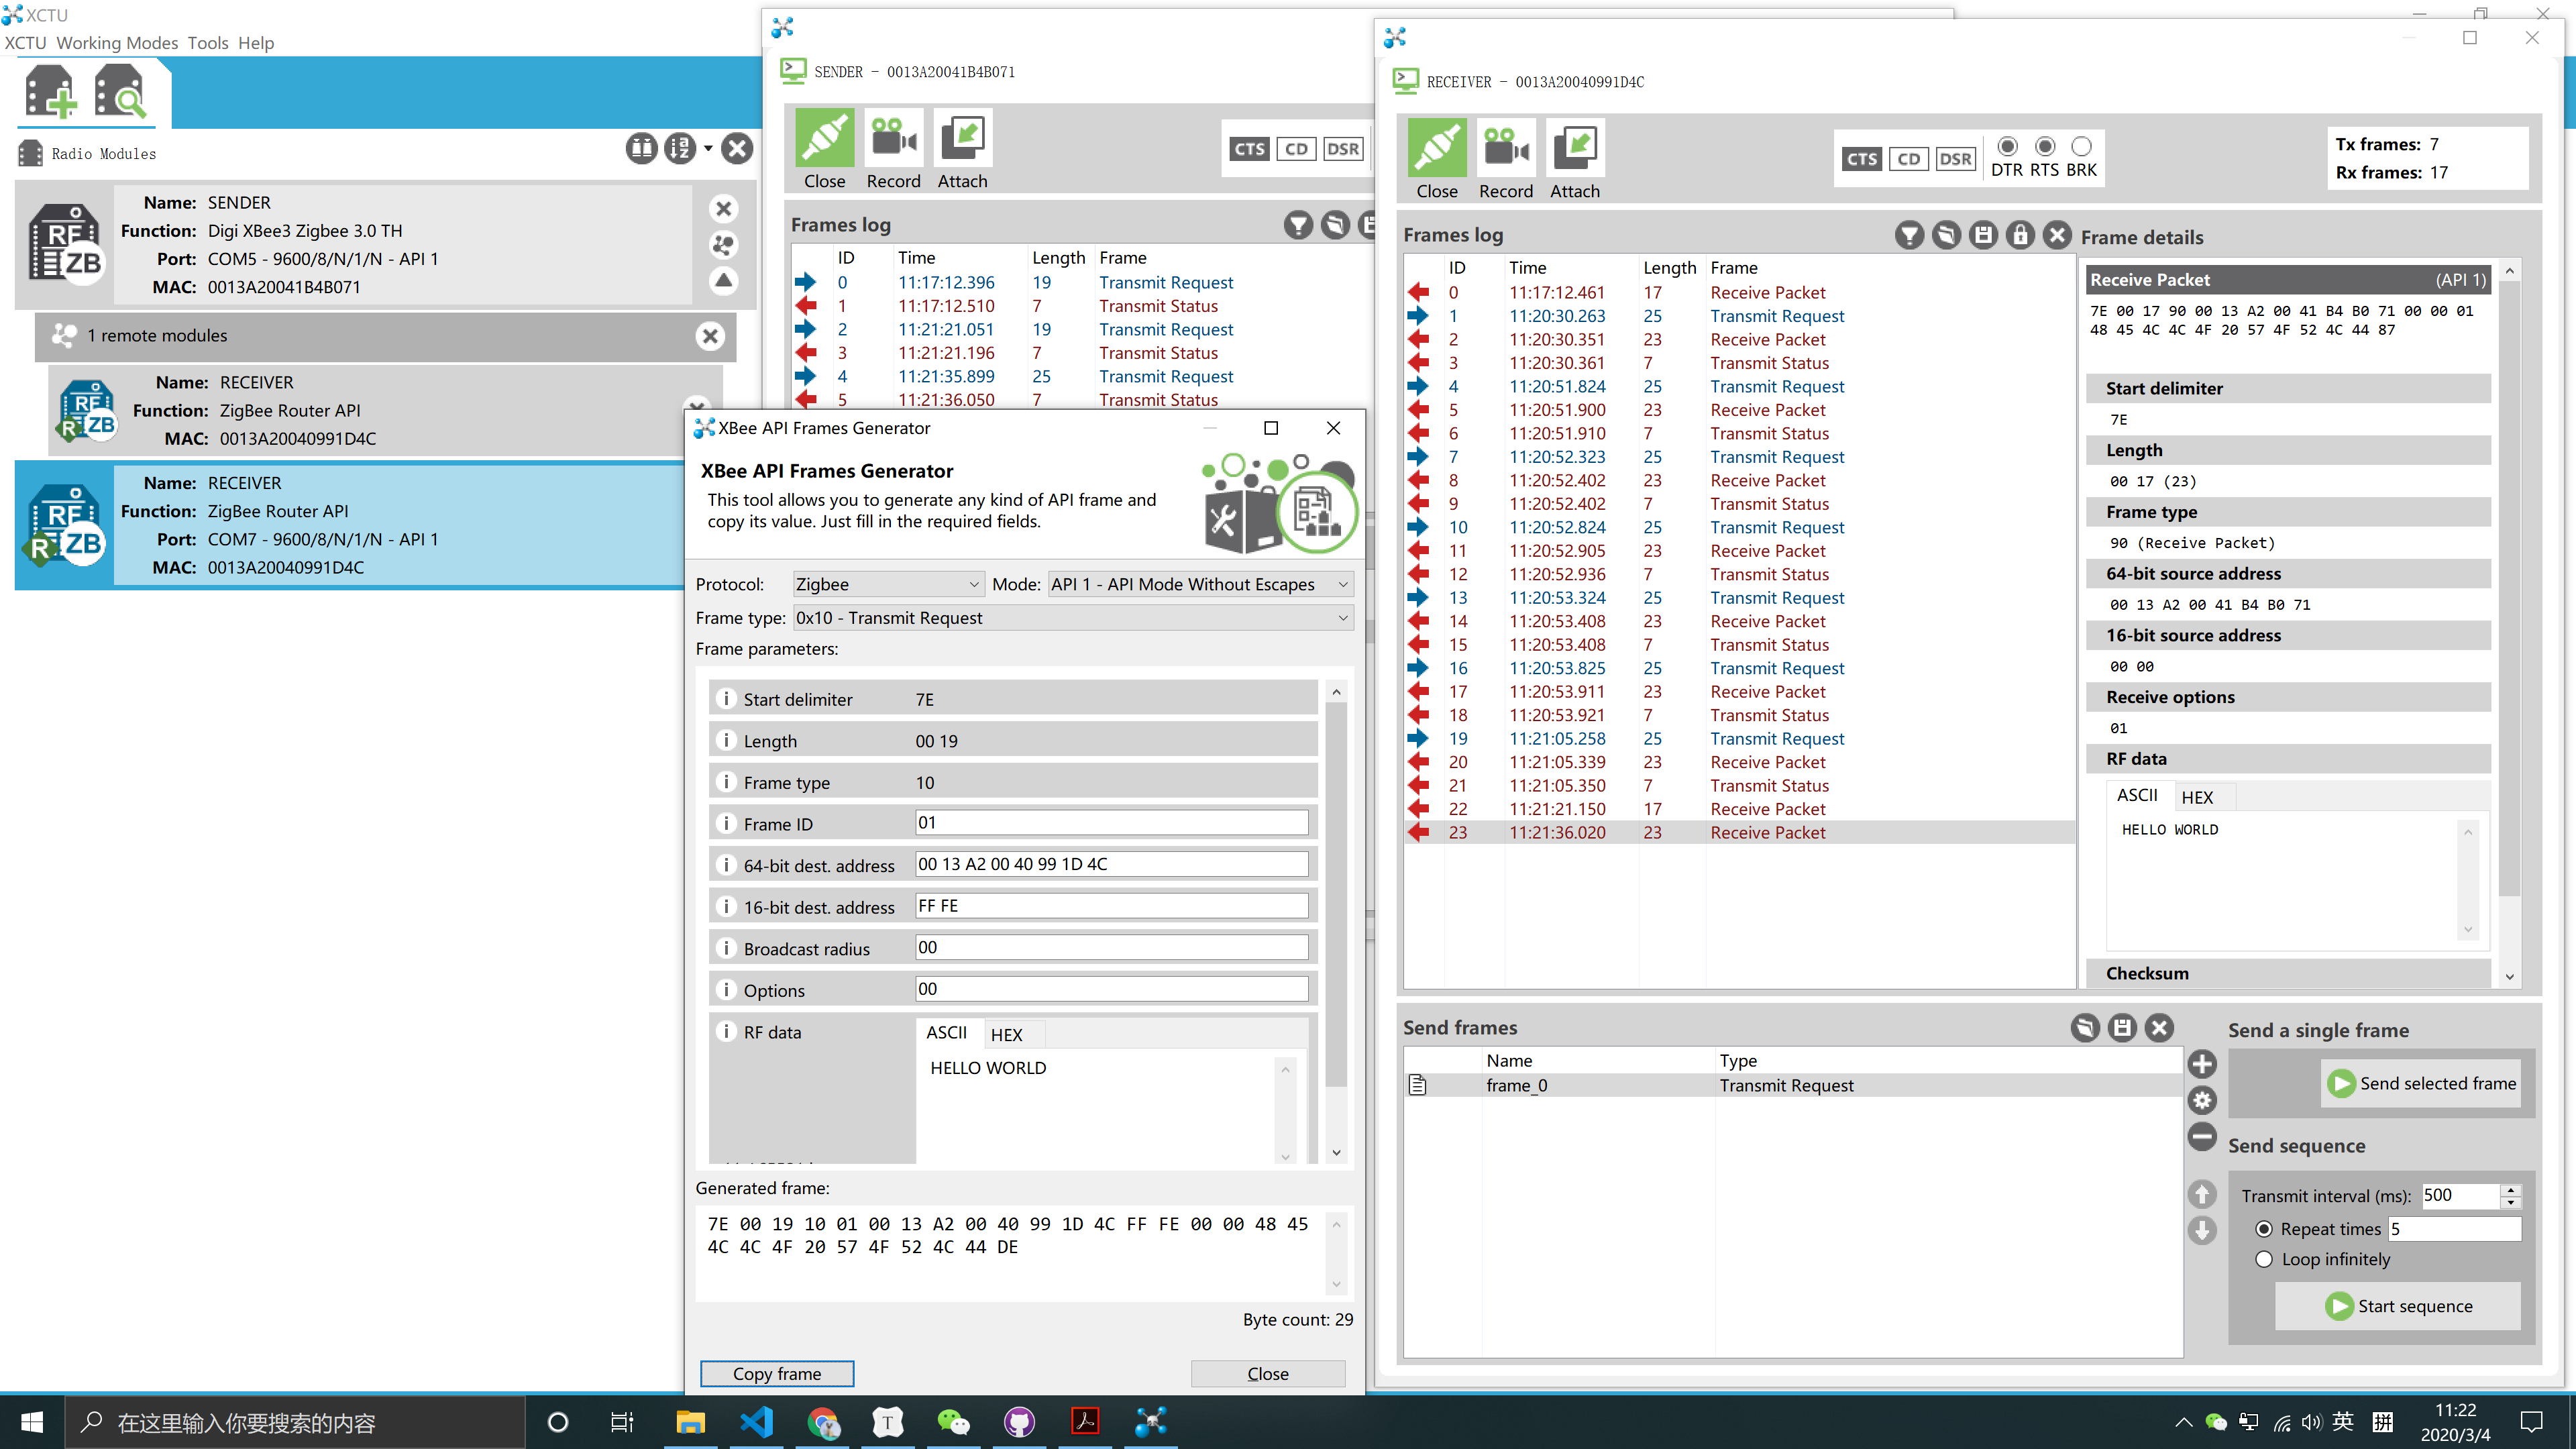
\includegraphics[width=\columnwidth]{XBee-XTCU-Send-Frame.png}
    \caption{XTCU发送Transmit Request frame}
    \label{fig:XBee-XTCU-Send-Frame}
\end{figure}


\subsection{XCTU参数设置}

coordinator是中心节点,Router是小机器人的,他们的配置要注意,比如AP=2,DH/DL是地址,都设为零,因为按照api里定义的地址发送,配置里的目的地址就填零就行。配置如表~\ref{tab:XCTU}所示。

% Please add the following required packages to your document preamble:
% \usepackage{booktabs}
\begin{table}[htbp]
    \centering
    \begin{tabular}{@{}lllll@{}}
    \toprule
    Param  & 全称  & Coordinator & Router & 作用 \\ \midrule
    ID &  Extended PAN ID      &  0                    & 0                   & 定义模块要连接的网络名称,所有模块的网络ID相同即可 \\
    JV &  Channel Verification &  —                    & Enabled{[}1{]}      & 验证当前频道是否存在Coordinator,若不存在则退出 \\
    CE &  Device Role          &  Form Network {[}1{]} & —                   & 设置当前设备为Coordinator \\
    NI &  Node Identifier      &  SENDER               & RECEIVER            & 定义节点标识符,是模块显示的名称,默认是一个空格,注意删除 \\
    AP &  API Enable           &  API Enabled {[}1{]}  & API Enabled {[}1{]} & 使能API模式 \\ \bottomrule
    \end{tabular}
    \caption{XCTU配置}
    \label{tab:XCTU}
\end{table}

\subsection{打开XCTU console}

\begin{enumerate}
    \item 切换到控制台工作模式。
    \item 打开与无线电模块的串行连接。
    \item 转到另一个XBee模块的控制台。
    \item 打开与无线电模块的串行连接。
\end{enumerate}

\subsection{生成Transmit Request frame}

使用XCTU SENDER console生成Transmit Request frame,如图~\ref{fig:XBee-XTCU-Generate-Frame}。

\begin{figure}[htbp]
    \centering
    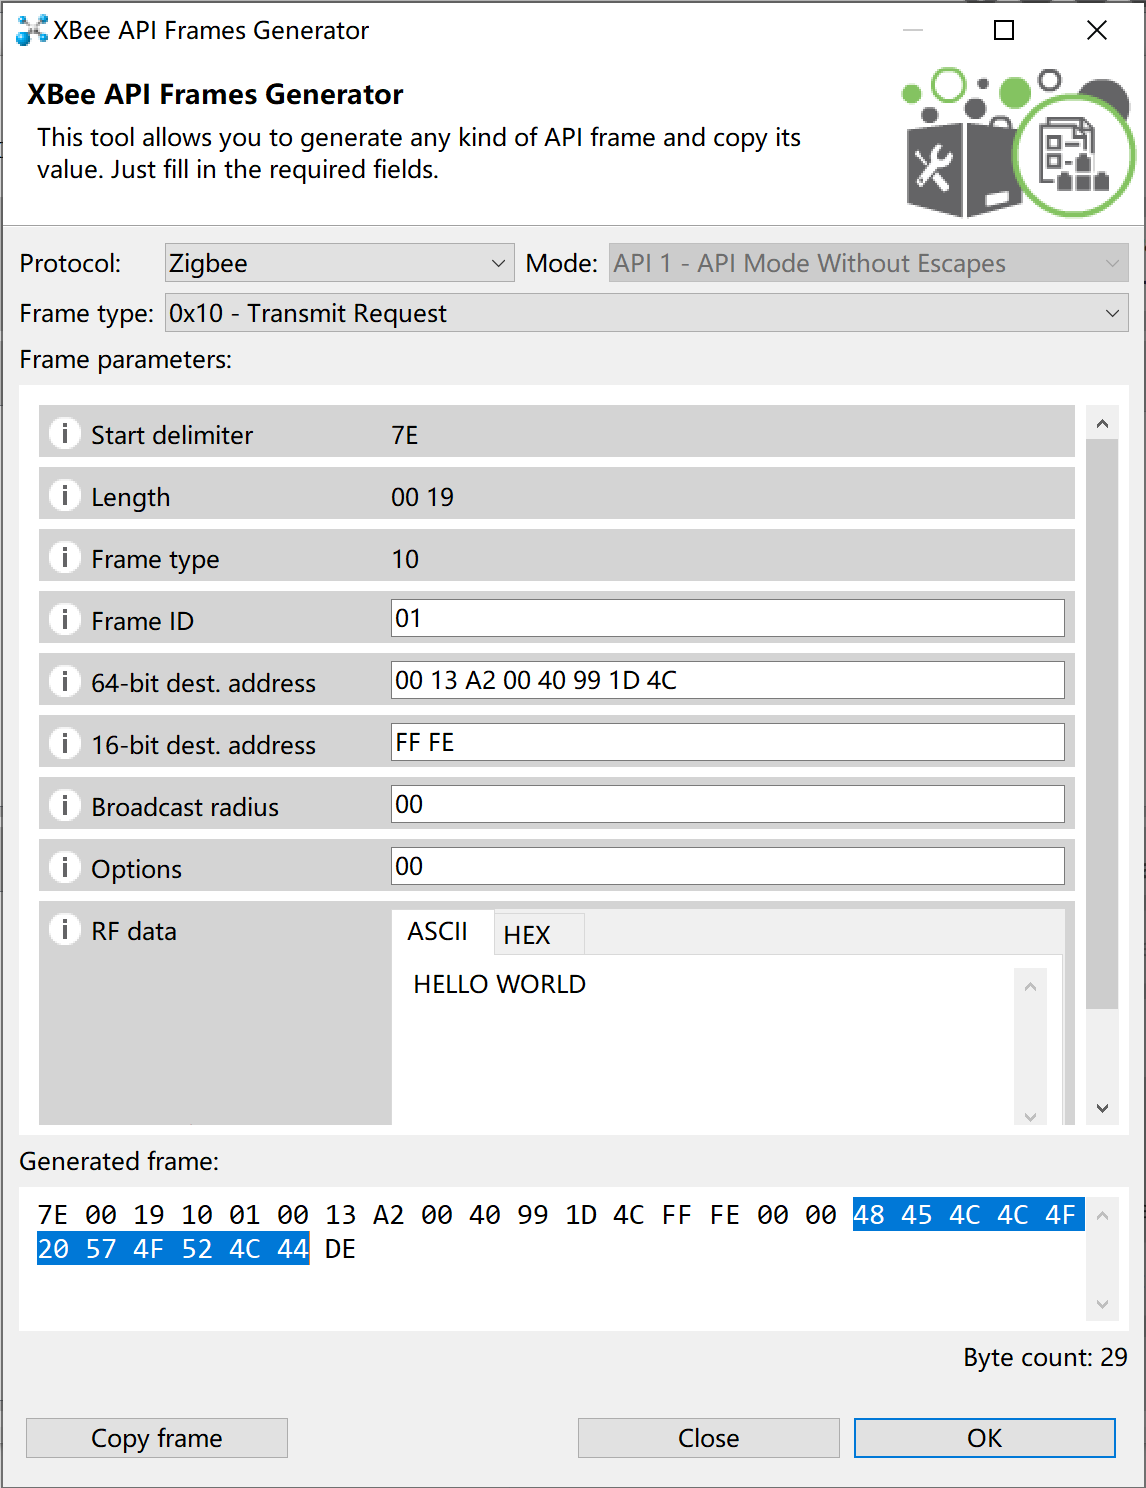
\includegraphics[width=0.8\columnwidth]{XBee-XTCU-Generate-Frame.png}
    \caption{XTCU生成Transmit Request frame}
    \label{fig:XBee-XTCU-Generate-Frame}
\end{figure}

\begin{enumerate}
    \item 使用Detach分离Console 以同时查看两个控制台
    \item 在SENDER console中点击Add new packet to the list
    \item 打开Frames Generator tool
    \item Protocol control选Zigbee
    \item Frame type control 选 0x10 - Transmit Request
    \item 在64-bit dest. address中输入RECEIVER module的64-bit地址
    \item 在RF data中选中ASCII选项卡并输入信息"Hello, this is SENDER!"
    \item 点OK
    \item 点Add frame
\end{enumerate}

\subsection{发送Transmit Request frame}

点Send selected packet

Frames log指示已发送一个帧(蓝色),而已接收另一个帧(红色)。

\subsection{分析}

\begin{tcolorbox}
    Transmit Request (API 1)
    \\ 
    \\ 7E 00 19 10 01 00 13 A2 00 40 99 1D 4C FF FE 00 00 48 45 4C 4C 4F 20 57 4F 52 4C 44 DE
    \\ 
    \\ Start delimiter: 7E
    \\ Length: 00 19 (25)
    \\ Frame type: 10 (Transmit Request)
    \\ Frame ID: 01 (1)
    \\ 64-bit dest. address: 00 13 A2 00 40 99 1D 4C
    \\ 16-bit dest. address: FF FE
    \\ Broadcast radius: 00 (0)
    \\ Options: 00
    \\ RF data (HEX): 48 45 4C 4C 4F 20 57 4F 52 4C 44
    \\ RF data (ASCII): HELLO WORLD
    \\ Checksum: DE
\end{tcolorbox}

Transmit Request (API 1)如图~\ref{fig:XBee-XTCU-Sender-Transmit-Request}。

\begin{figure}[htbp]
    \centering
    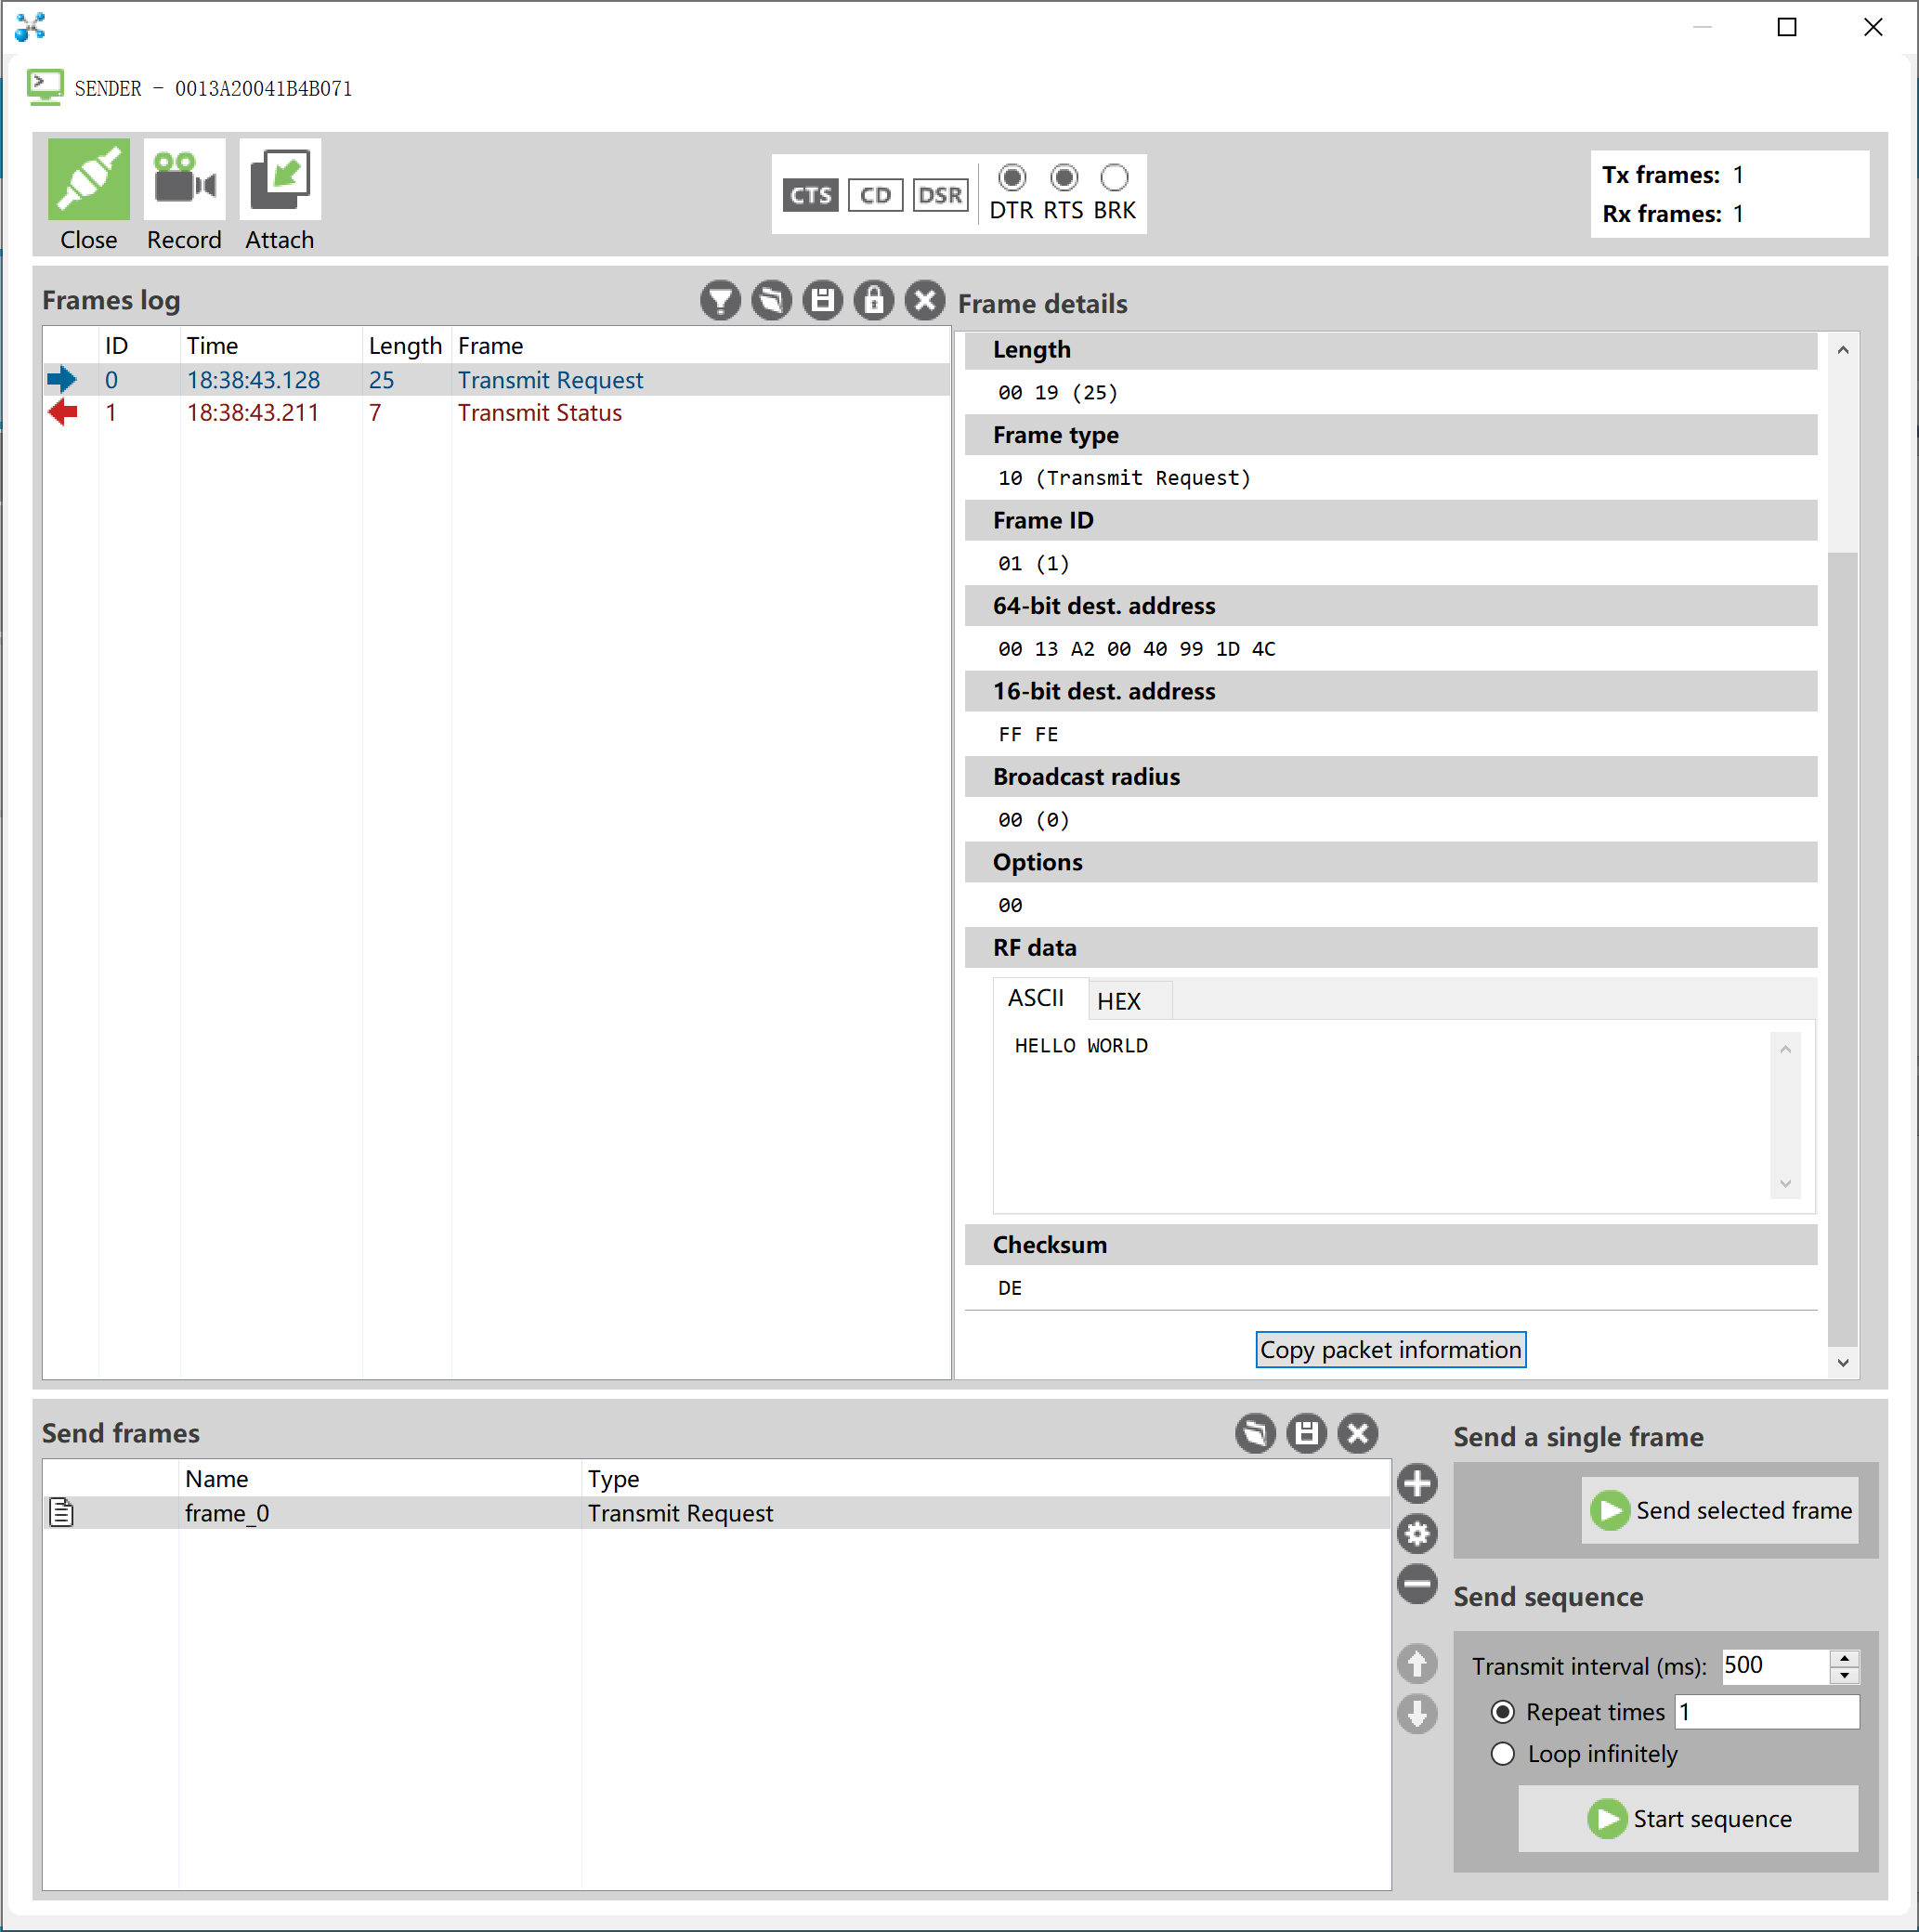
\includegraphics[width=0.8\columnwidth]{XBee-XTCU-Sender-Transmit-Request.png}
    \caption{XTCU Transmit Request}
    \label{fig:XBee-XTCU-Sender-Transmit-Request}
\end{figure}

\begin{tcolorbox}
    Transmit Status (API 1)
    \\ 
    \\ 7E 00 07 8B 01 99 09 00 00 00 D1
    \\ 
    \\ Start delimiter: 7E
    \\ Length: 00 07 (7)
    \\ Frame type: 8B (Transmit Status)
    \\ Frame ID: 01 (1)
    \\ 16-bit dest. address: 99 09
    \\ Tx. retry count: 00 (0)
    \\ Delivery status: 00 (Success)
    \\ Discovery status: 00 (No discovery overhead)
    \\ Checksum: D1
\end{tcolorbox}

Transmit Status (API 1)如图~\ref{fig:XBee-XTCU-Sender-Transmit-Status},表明此帧信息被成功发送。

\begin{itemize}
    \item Frame type: 8B (Transmit Status) 说明这是发送之后本机返回的发送状态信息。
    \item Frame ID: 01 (1) 因为 Transmit Request 和 Transmit Status 有相同的ID,说明这是前一条 Transmit Request 的发送状态。
    \item Delivery status: 00 (Success) 说明这条消息发送成功了。
\end{itemize}

\begin{figure}[htbp]
    \centering
    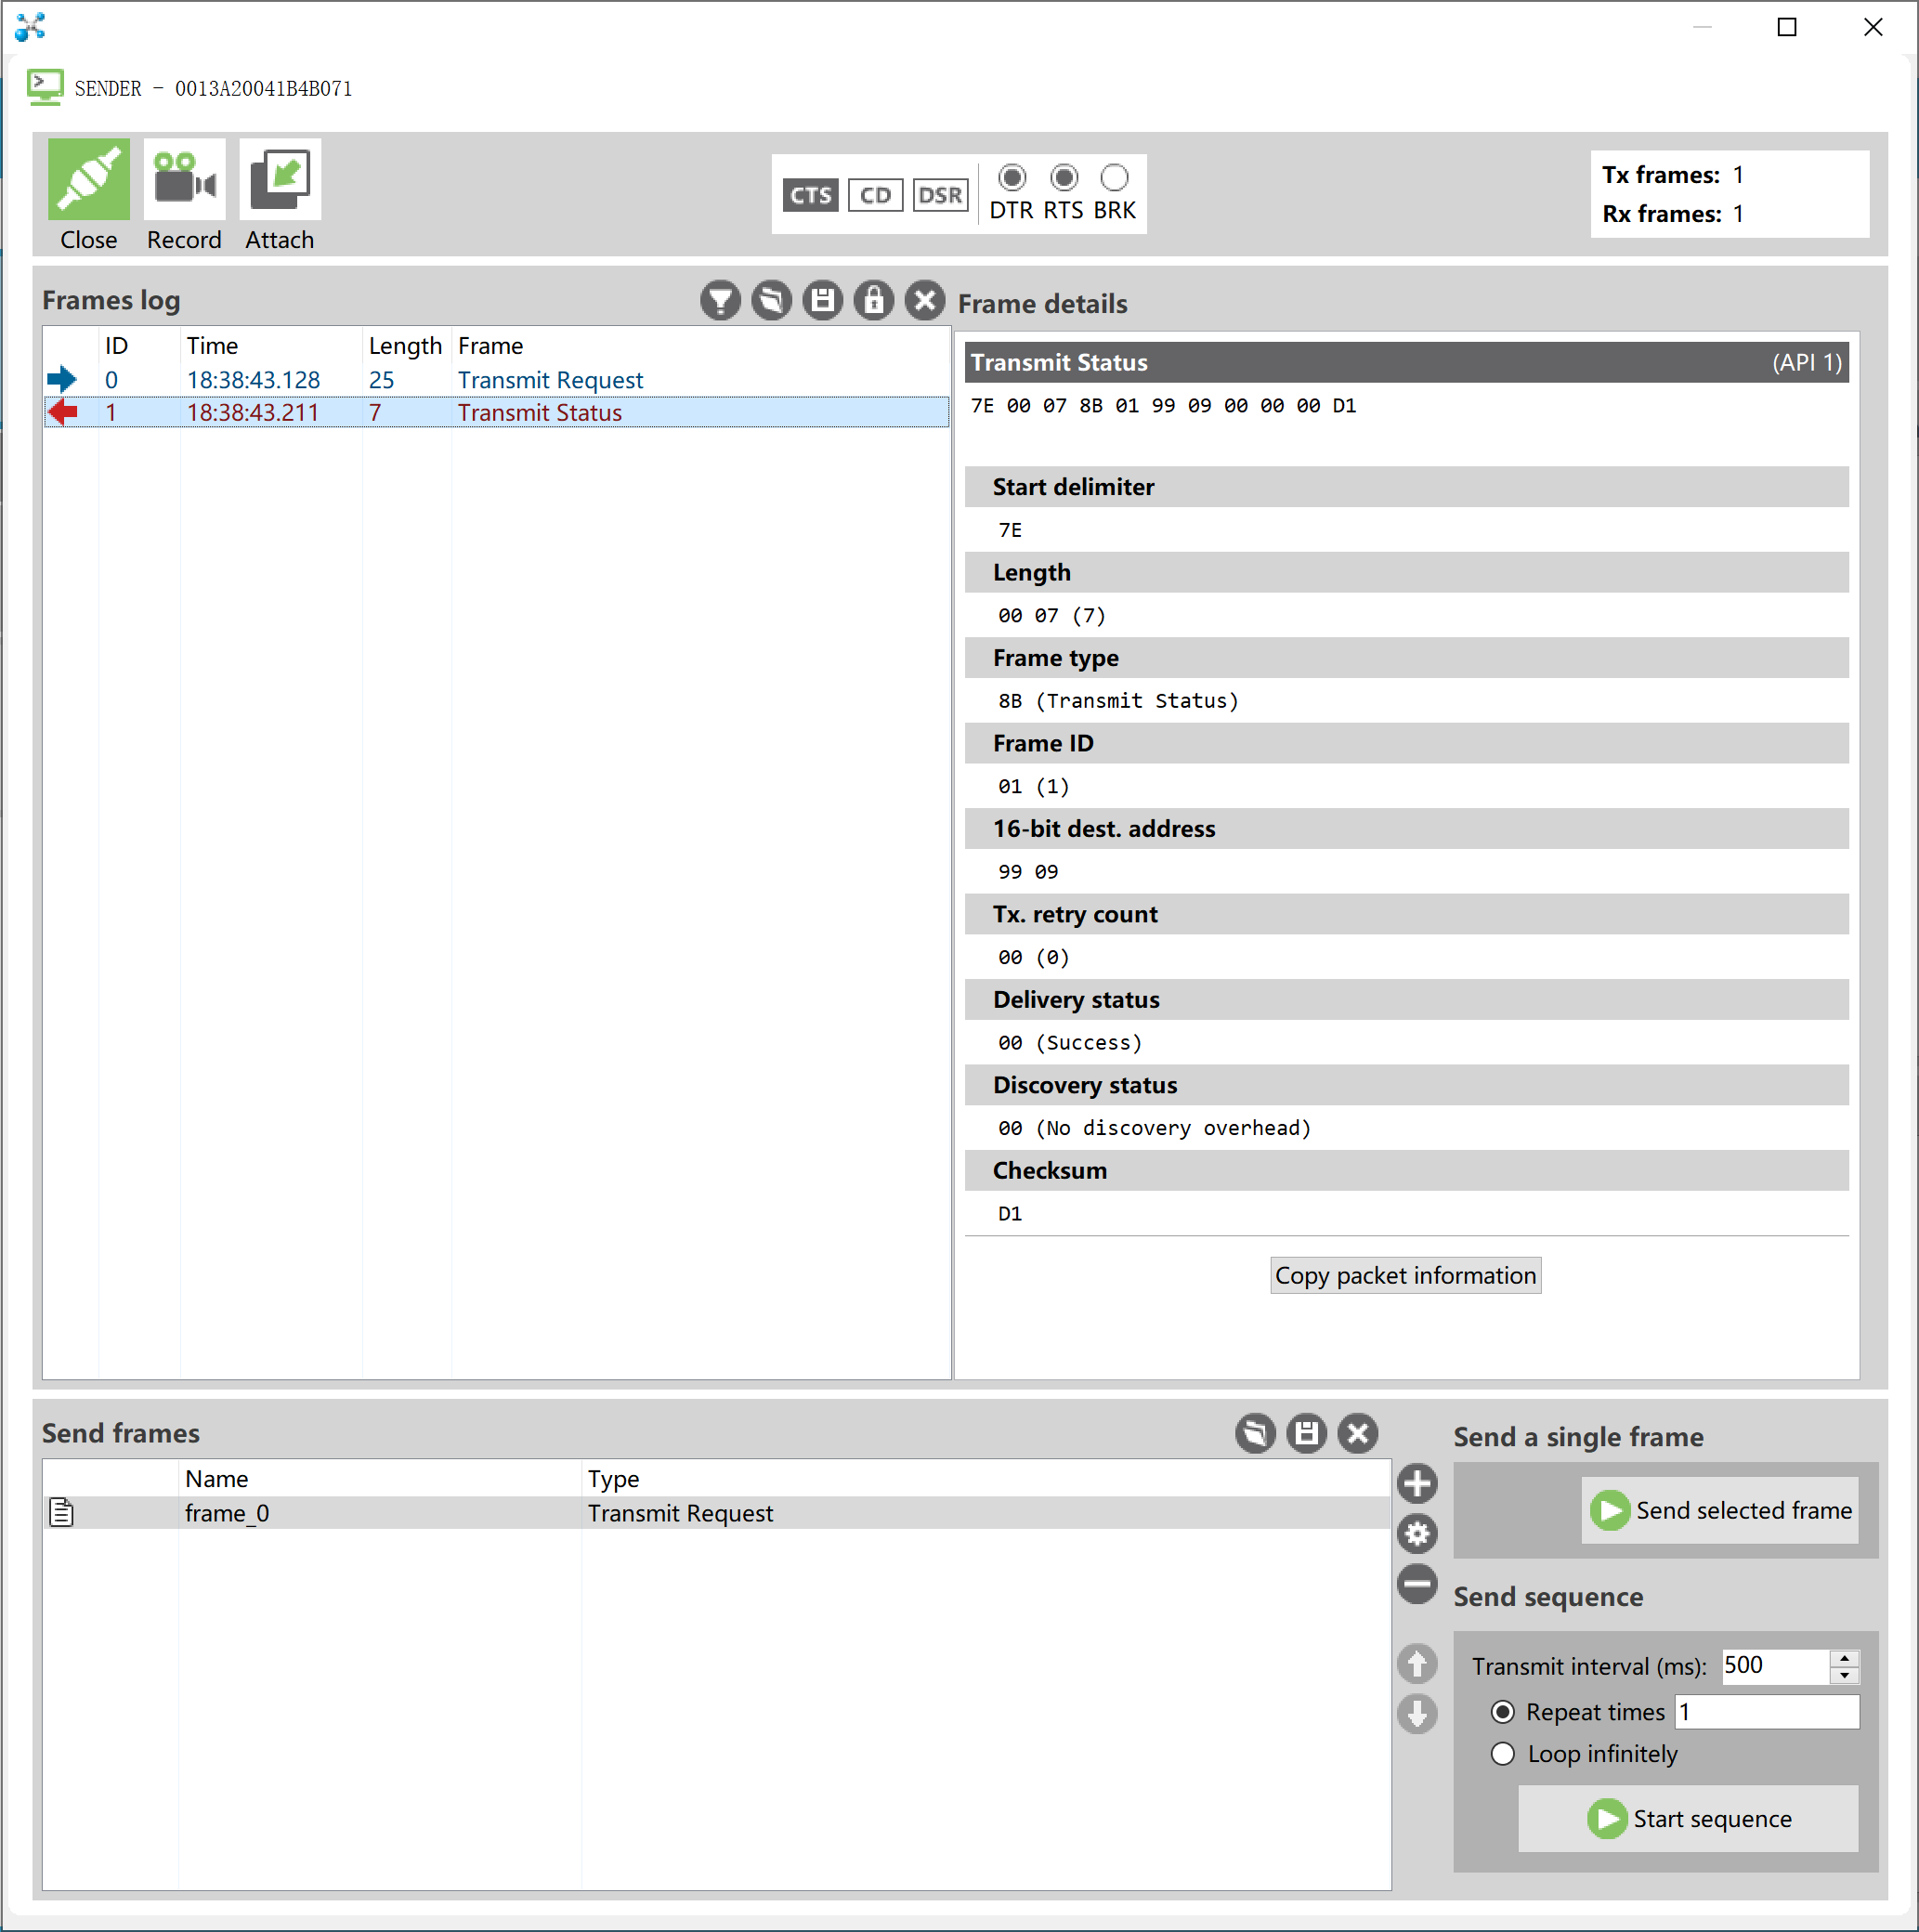
\includegraphics[width=\columnwidth]{XBee-XTCU-Sender-Transmit-Status.png}
    \caption{XTCU Transmit Status}
    \label{fig:XBee-XTCU-Sender-Transmit-Status}
\end{figure}

\begin{tcolorbox}
    Receive Packet (API 1)
    \\ 
    \\ 7E 00 17 90 00 13 A2 00 41 B4 B0 71 00 00 01 48 45 4C 4C 4F 20 57 4F 52 4C 44 87
    \\ 
    \\ Start delimiter: 7E
    \\ Length: 00 17 (23)
    \\ Frame type: 90 (Receive Packet)
    \\ 64-bit source address: 00 13 A2 00 41 B4 B0 71
    \\ 16-bit source address: 00 00
    \\ Receive options: 01
    \\ RF data (HEX): 48 45 4C 4C 4F 20 57 4F 52 4C 44
    \\ RF data (ASCII): HELLO WORLD
    \\ Checksum: 87
\end{tcolorbox}


Receive Packet (API 1) 如图~\ref{fig:XBee-XTCU-Receive-Packet}。分析RECEIVER的接收数据包的详细信息。 确认是刚刚输入的信息"HELLO WORLD",并且发件人的地址是SENDER。

\begin{itemize}
    \item Frame type: 90 (Receive Packet) 说明这是接收到的数据包
    \item 64-bit source address 是SENDER的64-bit地址
    \item Receive options: 01 The packet was acknowledge (0xC1 = 1100 0001)
    \item RF data (ASCII): HELLO WORLD 数据包内的信息是"HELLO WORLD"
\end{itemize}

\begin{figure}[htbp]
    \centering
    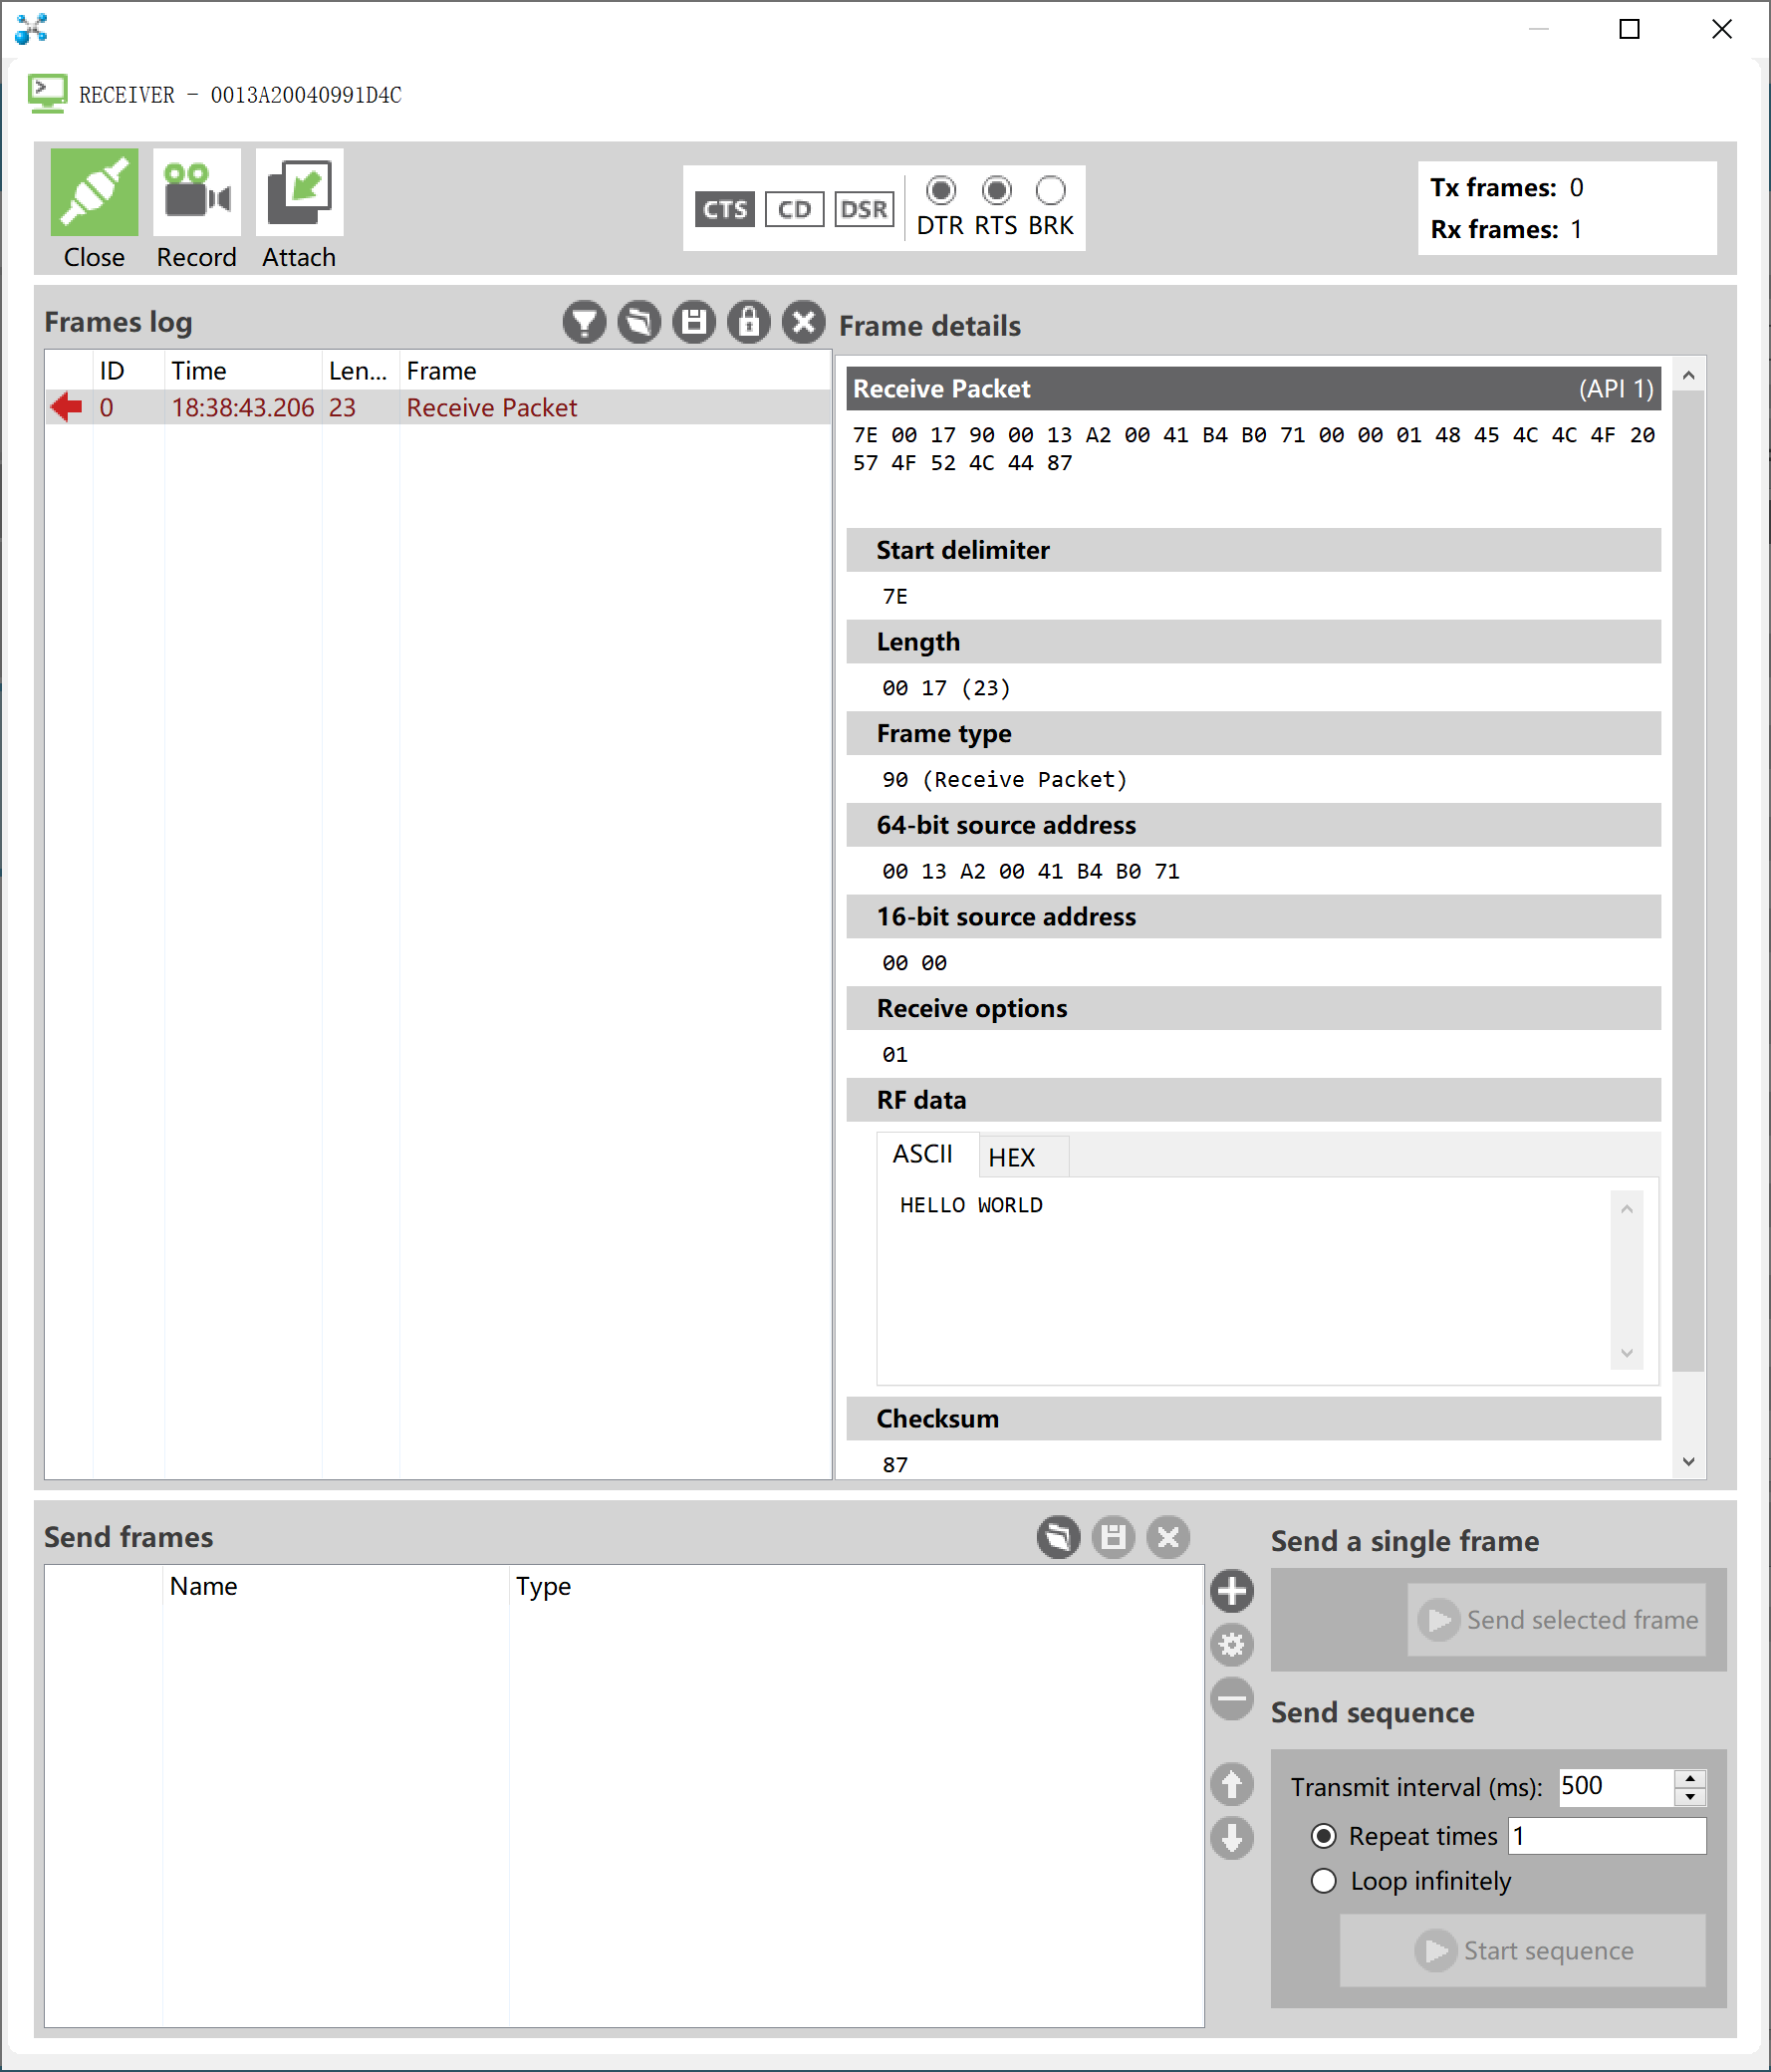
\includegraphics[width=\columnwidth]{XBee-XTCU-Receive-Packet.png}
    \caption{XTCU Receive Packet}
    \label{fig:XBee-XTCU-Receive-Packet}
\end{figure}


\section{Arduino XBee 开发环境配置}

在库管理器中安装 xbee-arduino library \footnote{\url{https://github.com/andrewrapp/xbee-arduino}} 。

MsTimer2 and FlexiTimer2 Libraries \footnote{\url{https://www.pjrc.com/teensy/td_libs_MsTimer2.html}}

\section{ARM开发环境配置}

XBee mbed Library \footnote{\url{https://developer.mbed.org/teams/Digi-International-Inc/code/XBeeLib/}}是现成的mbed扩展,用于在mbed平台上开发XBee项目。